% LaTeX file for Chapter 01



%  possible title: Causal inference for non-randomized data and heterogeneous treatment effect estimation


\chapter{Introduction}

% Why, what and how\dots

The important questions that studies want to answer are usually not associational but causal \citep{pearl2009}. For example, these are questions that ask for effects when making a certain intervention, like the effect of a treatment. They can ask for reasons that lead to the observed outcome, like which disease caused the given symptoms. Or what would have been different if another action was taken, like what would the GDP have been, if the interest rates were incereased only by 25 instead of 75 Bps. To answer such questions, a causal reasoning must be applied that aims to understand the underlying data genearting mechanism, sole associational reasoning directly from the data is not sufficient. 


% https://ascpt.onlinelibrary.wiley.com/doi/epdf/10.1002/cpt.3159
% One of the main reasons for this is thatML methods are particularly good at learning about the status quofrom existing data to ultimately make outcome predictions thatare exactly in line with the current distribution of data character-istics, but usually not designed for tasks that involve the need toreason about interventions on the data generating distributionsleading to counterfactual scenarios,


\textbf{Importance of Causal Inference on Observational Data}


The gold standard to measure causal relationships between an intervention and an outcome is the randomized controlled trial (RCT) \citep{hariton2018}. The key concept of this prospective study design, is that the participants are randomly allocated due either the treatment or control group. Due to this randomization, the influence of potential confounding variables is eliminated and study groups are balanced with respect to baseline characteristics allowing for an unbiased cause-effect estimation.
Disadvantages of RCTs include but are not limited to often high cost, the time for planning and executing the trial, and generalisability to the population of interest. % (from paper: participants that volunteer to participate might not be representative of the population being studied)
Furthermore, RCTs typically aim to estimate an average treatment effect on a sample, which is the difference in the averages accross the treatment groups \citep{nichols2007}. However, patients have individual responses to the treatment, depending on their characteristics. In personalized medicine, such individual treatment effects are crucial.
Another central limitation of RCTs is that in many scenarios they can not be conducted due to ethical or practical reasons. For example, an RCT is only ethical in the case of clinical equipoise, which means that there is uncertainty about the (superiority) of one of the two treatment arms \citep{freedman1987}. It is not acceptable to treat one group with the assumed inferior treatment. The same is true for obviously harmful interventions, like smoking or drinking alcohol. In these cases, it is not possible to conduct an RCT to estimate the causal effect of smoking on lung cancer.

Therefore, much of the research aims to make causal inference from observational data in a non-experimental or quasi-experimental design. In an observational setting, there are usually confounding variables that make it challenging to measure the effect between exposure and outcome. Methods for causal infreence on observational data for example aims to correctly adjust or control for confounders. \citet{sick2025} proposed the framework of TRAM-DAGs to estimate the causal relationships in an observational setting and make subsequent queries. The aim of this thesis is to further analyze this method and apply it in a real-world scenario.


\textbf{General Causality review (DAG, SCM, Pearls ladder, rubins rules?)}

Causal relationships can be represented by a directed acyclic graph (DAG) as, for example, shown in Figure \ref{fig:pearl_levels}(a). The variables, or nodes, are connected by directed edges which indicate the path of causal dependence.

Usually we want to answer questions that can be assigned to one of the groups in pearls hierarchy of causation \citet{pearl_book2009}. Visual examples are presented in Figure \ref{fig:pearl_levels}(a)-(c). Level 1 are observational queries which are conditional probabilities $P(Y \mid X)$ and can be answered directly from the joint distribution $P(Y \cap X)$. Level 2 are interventional queries which are probabilities $P(Y \mid do(X))$ that result by a taken action do(X). Where observational queries only require to know the joint distribution, for interventional queries an additional understanding of the causal mechanism is necessary. Level 3, the analysis of counterfactuals, poses the biggest challenge. These are what-if questions. An example of this would be if a sick patient was treated with a certain treatment and then died. Death would therefore be the observed and therefore factual outcome. The counterfactual outcome is the outcome that would have occurred if the patient had received a different medication. Such counterfactual questions are often labelled as metaphysical because they can never be tested directly. However, there are important practical questions that require the analysis of such counterfactuals.



% include image /img/pearl_levels.png
\begin{figure}[H]
\centering
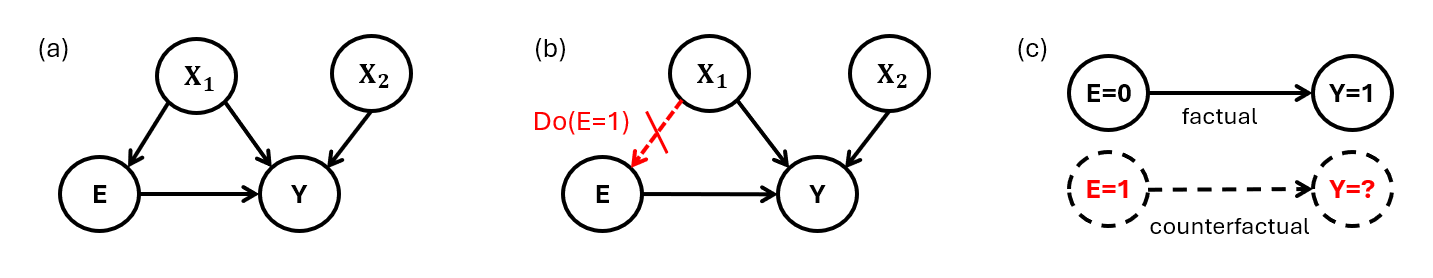
\includegraphics[width=1\textwidth]{img/pearl_levels.png}
\caption{Example for the three levels of Pearl's hierarchy of causation. (a) DAG for observational data. (b) DAG when making a do-intervention by fixing the variable E at a certain value. c) Observed factual outcome and corresponding counterfactual query.}
\label{fig:pearl_levels}
\end{figure}


To illustrate Pearl's three levels of causality, I consider a simplified example involving the exposure Exercise (E), the outcome Heart Disease (Y), the confounder Age ($X_1$) and the additional covariate Smoking ($X_2$). I assume that exercise reduces the risk of heart disease, but both variables are also influenced by age. Figure \ref{fig:pearl_levels}(a)-(c) illustrates the corresponding scenarios.

\textbf{Level 1: Observational ("seeing").}  
We observe the joint distribution of variables without intervention.  
Example: What is the probability of heart disease given that a person exercises?  
\[
P(Y \mid E = 1)
\]
This can be estimated directly from data (by filtering for E=1 and calculating the fraction of Y), but does not account for confounding.


\textbf{Level 2: Interventional ("doing").}  
We consider the effect of an intervention on the system.  
Example: What is the probability of heart disease if everyone were made to exercise, regardless of age or smoking?  
\[
P(Y \mid \text{do}(E = 1))
\]
This requires assumptions about the causal structure.


\textbf{Level 3: Counterfactual ("imagining").}  
We ask what would have happened under different circumstances, which means imagine an alternative reality.
Example: For a person who does not exercise and has heart disease, would they still have heart disease if they had exercised?  
\[
P(Y_{E=1} \mid E = 0, Y = 1)
\]
Here $Y_{E=1}$ is the outcome under the positive exposure. Counterfactual queries require a structural causal model and cannot be answered from data alone.


% With our new framework, we can answer all three types of questions, with a small exception for Counterfactuals in the non-continuous case.




\textbf{What is a Structural Causal Model?}
% pearl book p. 27
To answer questions from Pearl's ladder of causation, the concept of DAG's can be extended to structural causal model (SCM). A set of structural equations of the from $x_i = f_i(pa(x_i), z_i)$, $i=1,...,n$ forms a structural causal model \citep{pearl_book2009}. $pa(x_i)$ are the direct causal parents of $X_i$ and therefore directly determe its value. $Z_i$ are errors that follow exogeneous noise distributions $P(Z_i)$. They can be understood as latent variables that represent unmodeled factors which can not be observed or measured directly. By convention, the $Z_i$ are assumed to be mutually independent. % then by definition a markovian model
The potentially nonlinear function $f_i$ determines the functional form of the parents and the noise that represents the data generating mechanism of the dependent variable $X_i$. Hence, in a SCM a source node $X_j$ can be represented as $X_j = f_j(z_j)$ since it does not depend on any other variables in the system. Once all components of the structural equations are known (or assumed to be known), it is fully deterministic. 
% check Pearl p. 31. at the top. can i write it like this?

This representation makes it practical to determine interventional distributios and counterfactual queries. This will be discussed in detail in Section XXX.

%  described in pearl book 2009, p. 41+
In this thesis, the focus is not on finding the causal structure of a system. Such a structure can be found by structure finding algorithms, or determided by expert knowledge, for example. Instead, I assume the DAG to be known and focus on the estimation of the functional form of the relationships.

There is a variety of methods that are applied to quantify these structural equations that form the resulting SCM. 

% \[
% X_i = \beta_0 + \beta_1 X_{pa(x_i)} + Z_i
% \]
% 
% \[
%   X \sim \mathcal{N}(\mu = pa(X)\beta,\,\sigma^{2})\,.
% \] 


The simplest method might be the linear regression which assumes gaussian error terms $Z_i$ and a linear $f_i$. Similarly other classical statistical methods can be applied they have the advantage of being typically well defined and having interpretable parameters. However, they require to make strong assumptions about the underlying data generating mechanism which can make them susceptible to bias if these assumptions are violated.

Then there is also the possibility to model the relationships with various methods based on neural networks. Because they can be very flexible, they can also model complex underlying distributions with practically no bias. But this comes at the cost of less interpretability. And often they are limited to continuous data.
% make this part more thorough and add specific models and citations

The framework of TRAM-DAGs proposed by \citet{sick2025} builds a bridge between these two approaches of classical statistical and deep learning methods. It allows us to model the causal relationships with interpretable or fully-flexible parts, depending on what is regarded more important at the moment. The basis of this model is to construct the structural equations as transformation models as introduced by \citet{hothorn2014}, which is a flexible distributional regression method. To make them even more customizable, these transformation models (TRAMS) were extended to deep TRAMS \citep{sick2020}. Applied in a causal context, these deep TRAMS form the framework of TRAM-DAGs that can be fitted on observational data and allow to tackle causal queries on all three levels of Pearl's causal hierarchy. This framework will be explained in detail in the Section XXX.



The first goal of this thesis is to further analyze and extend TRAM-DAGs. This includes the application of TRAM-DAGs in different scenarios, such as different datatypes, level of complexity or Neural Network structures (activation function, batchnormalization, dropout). Most analyses are performed in simulation studies, but the model was also applied on real-world climate data.


An application where causal inference is of particular importance is the estimation of individualized treatment effects (ITE) or also referred to conditional average treatment effect (cATE) or uplift modelling often in a marketing context. They can be understood in the difference in outcomes under different treatments, on an individual or subgroup level. The idea is that they can be used for example in personnalized medicine or for targeted direct marketing campaigns. Each individual patient might respond differently to a specific treatment, depending on his unique characteristics. RCTs traditionally are used to estimate an average treatment effect (ATE) which might indicate the trend in the analyzed population, but the ITEs might be very different for individual patients. In the marketing context this individual effect is of high interest because marketing campaings can be executed very specific and individualized. For example, in the assessment wheter a certain customers should receive a push notification (treatment) or not. Here each customer could be attributed to one of 4 categories, the persuadables (if receiving a notification, they will buy a product or service), the sure thing (they will buy the product either way), the lost causes (they will not buy, regardless of receiving a notification or not), or the sleeping dogs (they will eventually buy, but not if they were treated). Therefore it is crucial to know for each (potential) customer, how he might respond to the treatment, the persuadables should definetely be treated so that we gain them as a customer and the sleeping dogs shall not receive one as we would loos them as customers. There exists many approaches and methods to estimate these individualized treatment effects. However, this is more difficult compared to sole predictive modelling. \citet{chen2025} showed that all causal machine learning models that were trained on a train set failed to generalize to a test set. 

Analyzing what could be the reason for this behaviour and potential solutions constitute the second goal of this thesis. With the help of simulaition studies we evalueate scenarios when the estimation of ITE fails. Furthermore we show that TRAM-DAGs can be used to estimate the ITE, also in a non-RCT setting, as long as the data can be described by a fully observed DAG.







